%%%%%%%%%%%%%%%%%%%%%%%%%%%%%%%%%%%%%%%%%
% Short Sectioned Assignment LaTeX Template Version 1.0 (5/5/12)
% This template has been downloaded from: http://www.LaTeXTemplates.com
% Original author:  Frits Wenneker (http://www.howtotex.com)
% License: CC BY-NC-SA 3.0 (http://creativecommons.org/licenses/by-nc-sa/3.0/)
%%%%%%%%%%%%%%%%%%%%%%%%%%%%%%%%%%%%%%%%%

%----------------------------------------------------------------------------------------
%	PACKAGES AND OTHER DOCUMENT CONFIGURATIONS
%----------------------------------------------------------------------------------------

\documentclass[paper=a4]{article} % A4 paper and 11pt font size


\usepackage[hmargin=3.5cm]{geometry}
% ---- Entrada y salida de texto -----

\usepackage[T1]{fontenc} % Use 8-bit encoding that has 256 glyphs
\usepackage[utf8]{inputenc}

%\usepackage{fourier} % Use the Adobe Utopia font for the document - comment this line to return to the LaTeX default

% ---- Idioma --------

\usepackage[spanish, es-tabla]{babel} % Selecciona el español para palabras introducidas automáticamente, p.ej. "septiembre" en la fecha y especifica que se use la palabra Tabla en vez de Cuadro

% ---- Otros paquetes ----
\usepackage[hidelinks]{hyperref} % Estilo para los enlaces
\hypersetup{
  colorlinks   = true, %Colours links instead of ugly boxes
  urlcolor     = blue, %Colour for external hyperlinks
  linkcolor    = black, %Colour of internal links
  citecolor   = blue %Colour of citations
}
\usepackage{url} % ,href} %para incluir URLs e hipervínculos dentro del texto (aunque hay que instalar href)
\usepackage{amsmath,amsfonts,amsthm} % Math packages
%\usepackage{graphics,graphicx, floatrow} %para incluir imágenes y notas en las imágenes
\usepackage{graphics,graphicx, float} %para incluir imágenes y colocarlas
\usepackage{wrapfig}

%Para incluir codigo
%\usepackage{minted}
	
% Para hacer tablas comlejas
%\usepackage{multirow}
%\usepackage{threeparttable}

%\usepackage{sectsty} % Allows customizing section commands
%\allsectionsfont{\centering \normalfont\scshape} % Make all sections centered, the default font and small caps

\usepackage{fancyhdr} % Custom headers and footers
\pagestyle{fancyplain} % Makes all pages in the document conform to the custom headers and footers
\fancyhead{} % No page header - if you want one, create it in the same way as the footers below
\fancyfoot[L]{} % Empty left footer
\fancyfoot[C]{} % Empty center footer
\fancyfoot[R]{\thepage} % Page numbering for right footer
\renewcommand{\headrulewidth}{0pt} % Remove header underlines
\renewcommand{\footrulewidth}{0pt} % Remove footer underlines
\setlength{\headheight}{13.6pt} % Customize the height of the header

\numberwithin{equation}{section} % Number equations within sections (i.e. 1.1, 1.2, 2.1, 2.2 instead of 1, 2, 3, 4)
\numberwithin{figure}{section} % Number figures within sections (i.e. 1.1, 1.2, 2.1, 2.2 instead of 1, 2, 3, 4)
\numberwithin{table}{section} % Number tables within sections (i.e. 1.1, 1.2, 2.1, 2.2 instead of 1, 2, 3, 4)

\setlength\parindent{0pt} % Removes all indentation from paragraphs - comment this line for an assignment with lots of text

\newcommand{\horrule}[1]{\rule{\linewidth}{#1}} % Create horizontal rule command with 1 argument of height


%------------------------------------------------------------------------
%	TÍTULO Y DATOS DEL ALUMNO
%------------------------------------------------------------------------

\title{	
\normalfont \normalsize 
\textsc{\textbf{Modelos de Computación (2016-2017)} \\ Grado en Ingeniería Informática \\ Universidad de Granada} \\ [25pt] % Your university, school and/or department name(s)
\horrule{0.5pt} \\[0.4cm] % Thin top horizontal rule
\huge Autómatas Celulares \\ % The assignment title
\horrule{2pt} \\[0.5cm] % Thick bottom horizontal rule
}

\date{\normalsize\today} % Incluye la fecha actual

%-------------------------------------------------------------------------
% DOCUMENTO
%-------------------------------------------------------------------------

\begin{document}

\maketitle % Muestra el Título

\newpage

%-------------------------------------------------------------------------
%	Resumen introductorio (entre 5 y 15 lineas)
%----------------------------------------------------------------------
\begin{abstract} 
% INCOMPLETO!!!!!
Se ha realizado un trabajo sobre los Autómatas Celulares desarrollados en la época de los 60 por \textit{Von Neumann}. La teoría de los Autómatas Celulares ha ido cambiando durante su vida con diferentes vertientes y multitud de variaciones pero nos centraremos en solo dos versiones más a parte de la de Von Neumann.

% IDEA BASICA Y GENERAL - HAY QUE HACERLO BIEN!!!!!!!!

\end{abstract}

%--------------------------------------------------------------------------
%	Introducción
%-------------------------------------------------------------------------

\section{Introducción} % 
% http://web.archive.org/web/20080907225701/http://yupana.autonoma.edu.co/publicaciones/yupana/005/autocelular/Automatas.html

%

Para poder entender que son los Autómatas Celulares primero debemos comprender de donde viene la necesidad de crearlos. En la historia del ser humano y las ciencias se ha perseguido el modelamiento del mundo y todos sus fenómenos que ocurren en el, en concreto de los sistemas físicos, eléctricos y mecánicos mediante el uso de los modelos matemáticos. Matemáticamente hablando, estos fenómenos de la naturaleza son sistemas de naturaleza continua y han sido tratados con ecuaciones diferenciales, integrales funcionales y variables de estado entre otros procedimientos matemáticos para su modelamiento. También están los modelos aproximados y discretos que ofrecen una teoría muy cercana a la realidad con la ventaja de utilizar valores finitos. Para ello se ha utilizado la discretización y la digitalización de sistemas.\\

Una de las técnicas matemáticas complejas para el modelado de sistemas físicos y mecánicos es el \textit{Método de los Elementos Finitos} (FEM), cuya finalidad es discretizar espacios de naturaleza continua, sobre los cuales es posible realizar análisis numéricos para comprender, por medio de un modelo discreto, el comportamiento de sistemas analógicos. Pero esta técnica resulta muy compleja de aplicar por su dificultad para poder lograr modelos que describan sus comportamientos de forma precisa. Esta técnica (FEM) tiene una alta aplicación en el análisis de sistemas y espacios físicos-mecánicos donde el objetivo del modelo es comprender el comportamiento del sistema en el ámbito de la resistencia de los materiales, la dinámica de partículas y en general el comportamiento con la interacción  de los elementos base del sistema en el espacio donde reside.\\

Aun así hay todavía un amplio grupo de sistemas que es imposible modelar con estas técnicas debido a diversos motivos, como por ejemplo, sistemas químicos, biológicos, evolutivos, eléctricos, computacionales e inclusive otros sistemas físicos y mecánicos. Para estos sistemas que no se podían modelar con FEM han aparecido a lo largo de la historia diferentes técnicas para obtener su modelo continuo, una de ellas fue el modelado con \textit{Autómatas Celulares}.




\section{Autómatas Celulares}
Aunque no existe una definición formal sobre que es un Autómata Celular entendemos que es un estudio de modelado discreto para un sistema que evoluciona en generaciones o iteraciones discretas. Es recomendable utilizar esta técnica cuando se tiene un sistema con una colección masiva de objetos simples que interactúan unos con otros de forma aleatoria y por ello es utilizado en la teoría de la computación, las matemáticas, la física, las ciencias complejas, etc. \\

Un Autómata Celular consiste en una rejilla regular de celdas, donde cada celda se conoce como célula y representa un estado del conjunto de estados disponibles del sistema. Cada celda puede tomar un valor de un rango de valores definidos para este sistema en particular, siempre que el valor sea discreto y perteneciente al conjunto de los reales. Además cada celda viene definida por su ``vecindario'', entendemos por vecindario al conjunto finito de las células adyacentes a una célula en concreto.  La rejilla va cambiando en el tiempo y actualizando el estado de sus células, a cada instante de tiempo se le denomina generación y el estado de las células en una generación no varía.  \\


En el autómata celular cuando se avanza de generación, se actualiza el valor de todas las células del autómata aplicando una función de transición (``evolución''), que avanza el autómata al estado siguiente. Esta función de transición viene determinada por una ecuación matemática que toma como argumentos los valores de la vecindad de la célula además de del valor de la propia célula. Siempre se aplica de forma homogénea y para cada paso discreto del tiempo.\\

Una manera de simular un autómata celular bidimensional es con una cuadrícula de tamaño infinito. Cada célula tiene dos posibles estados, viva o muerta. La vecindad de la célula se define por una regla en concreto, ya que la forma de considerar la adyacencia varía dependiendo del modelo y la versión del autómata que se utilice. Los tipos más comunes de vecindad son los que definieron \textit{Neumann} y \textit{Moore} y que se apodaron igual que sus autores. El vecindario definido por \textit{Von Neumann} se define como el conjunto de cuatro células que rodean ortogonalmente a una célula central. Hay una variante de este vecindario llamada ``zona ampliada de \textit{Von Neumann}'', que consiste en ampliar el vecindario a las ocho células que rodean ortogonalmente a la célula central. El vecindario definido por \textit{Moore} consiste en las ocho células adyacentes que rodean a una célula central.\\


\begin{figure}[H]
\centering
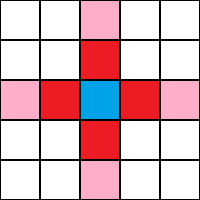
\includegraphics[scale=0.5]{imagenes/CA_Neumann.png}
\hspace{2cm}
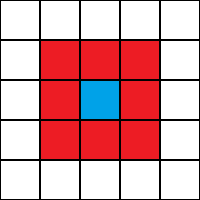
\includegraphics[scale=0.5]{imagenes/CA-Moore.png}
\caption{Vecindad en color rojo de la célula azul de forma gráfica, izquierda vecindad ampliada de Von Neumann y derecha vecindad de Moore.}
\label{fig:vecindad}

\end{figure}

La ecuación general del sistema de reglas que se utiliza para determinar el estado de la célula en la generación siguiente es del tipo $k^{k^s}$ donde $k$ es el número de posibles estados para una célula, y $s$ es el número de células de la vecindad (incluyendo al propia célula). De esta forma con la vecindad de \textit{Moore} en un sistema de dos dimensiones sería de $2^{2^9}$ el número total de autómatas posibles.\\

Los Autómatas Celulares se representaban con rejillas finitas en vez de las rejillas infinitas, ya que con la rejilla infinita no se podría realmente trabajar de forma precisa. Pero al utilizar una rejilla finita se presentaba una serie de problemas, el primero de ellos que tratamiento se realiza con las células de los bordes. Las células situadas en los limites de la rejilla ya no cuentan con una vecindad igual que el resto de las células del autómata, de esta forma la función de transición ya no trataría de la misma forma a todas las células. Si aplicamos una función  distinta a las células de los bordes no se estaría tratando tampoco de forma igualitaria a todas las células del autómata. Para este problema se han establecido unas soluciones llamadas ``condiciones frontera'', cada una de ellas esta orientada a solucionar distintos problemas reales del modelado:
\begin{itemize}
\item Frontera Abierta: Se considera que fuera de la rejilla residen células, todas con un valor fijo. En el caso particular de que el autómata tenga dos estados en su conjunto $k$, una frontera se dice fría si las células fuera de la frontera se consideran muertas, y caliente si se consideran vivas.
\item Frontera Periódica: Se considera a la rejilla como si sus extremos se tocaran. En una rejilla de dimensión 1, esto puede visualizarse en dos dimensiones como una circunferencia. En tres dimensiones la rejilla podría visualizarse como un toroide.

\begin{figure}[H]
\centering
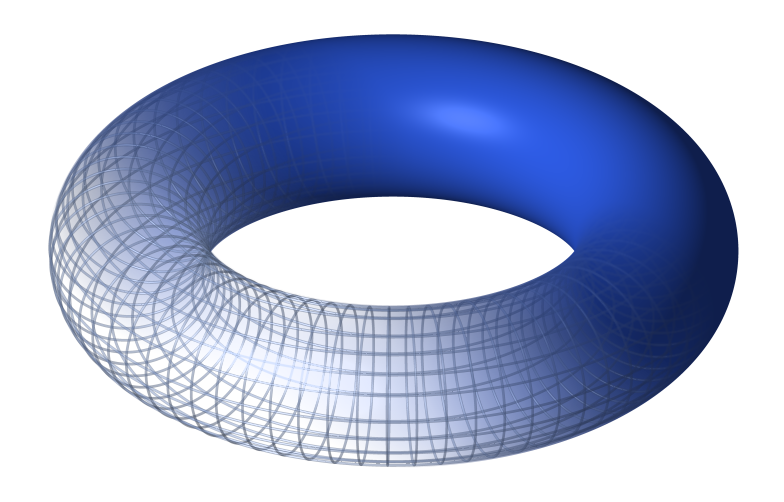
\includegraphics[scale=0.25]{imagenes/Torus.png}
\caption{Toroide, rejilla de Frontera Periodica en tres dimensiones.}
\label{fig:torus}
\end{figure}

\item Frontera Reflectora:  Se considera que las células fuera de la rejilla ``reflejan'' los valores de aquellas dentro de la rejilla. Así, una célula que estuviera junto al borde de la rejilla, por la parte de fuera tomaría como valor el de la célula que esté junto al borde de la rejilla, dentro de ella. 

 \item Sin Frontera: Haciendo uso de implementaciones que hagan crecer dinámicamente el uso de memoria de la rejilla implementada, se puede asumir que cada vez que las células deben interactuar con células fuera de la rejilla, esta se hace más grande para poder dar cabida a estas interacciones. Obviamente, existe un límite (impuesto por la memoria disponible) para esta condición. Es muy importante no confundir esta condición de frontera con la definición original de autómata celular cuya rejilla es inicialmente infinita. En el caso de un autómata celular sin frontera, la rejilla comienza con un tamaño definido y finito, y conforme se requiera va creciendo en el tiempo, lo cual no lo hace necesariamente un modelo más cercano a la realidad, pues si se inicializara la rejilla aleatoriamente, con esta condición sólo se pueden inicializar las células dentro de la rejilla inicial finita, mientras que en el caso de la definición original, en teoría todas las células de la rejilla infinita deberían ser inicializadas.
\end{itemize}


\subsection{Autómatas Celulares Lineales}
Unos de los Autómatas Celulares más utilizados y comunes son los denominados Autómatas Celulares lineales. Llamados así por que utilizan solo una dimensión, es decir, sus células están dispuestas una a continuación de otra a modo de una cadena. Si el autómata celular lineal consta de n células, cada una de ellas se nombrará por $\langle i \rangle$ con $ 0 = \leq i \leq n-1 $. Por ejemplo, un autómata celular lineal con cinco células sería:

\begin{figure}[H]
\centering
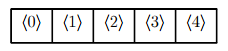
\includegraphics[scale=0.7]{imagenes/name_cell.png}
\label{fig:lineal_1}
\end{figure}

Si, además, $S_k$ es el conjunto de $k$ estados y $a_i^t \in S_k, \enspace 0 \leq i \leq n-1$, es el estado de la célula $\langle i \rangle$ en e instante $t$, entonces se denomina ``\textit{configuración del Autómata Celular en el instate $t$}'' y se denota por $C^t$ al siguiente vector:
$$C^t = \enspace \big( a_0^t,a_1^t, ..., a_{n-1}^t \big) \in S_k x ... n ... x S_k$$

La evolución de un autómata celular a lo largo del tiempo se representa de forma sencilla sin más que escribir las sucesivas configuraciones de sus células, una debajo de otra, a lo que llamaremos diagrama de evolución del autómata celular. A continuación se muestra un ejemplo del diagrama de evolución de un autómata celular de 5 células.

\begin{table}[H]
\centering
\begin{tabular}{lllllll}
\cline{1-5}
\multicolumn{1}{|l|}{$a_0^0$} & \multicolumn{1}{l|}{$a_0^1$} & \multicolumn{1}{l|}{$a_0^2$} & \multicolumn{1}{l|}{$a_0^3$} & \multicolumn{1}{l|}{$a_0^4$} & $\rightarrow$ & $C^0$ \\ \cline{1-5}
\multicolumn{1}{|l|}{$a_1^0$} & \multicolumn{1}{l|}{$a_1^1$} & \multicolumn{1}{l|}{$a_1^2$} & \multicolumn{1}{l|}{$a_1^3$} & \multicolumn{1}{l|}{$a_1^4$} & $\rightarrow$ & $C^1$ \\ \cline{1-5}
\multicolumn{1}{|l|}{$a_2^0$} & \multicolumn{1}{l|}{$a_2^1$} & \multicolumn{1}{l|}{$a_2^2$} & \multicolumn{1}{l|}{$a_2^3$} & \multicolumn{1}{l|}{$a_2^4$} & $\rightarrow$ & $C^2$ \\ \cline{1-5}
 &  & \multicolumn{1}{c}{...} &  &  &  & \multicolumn{1}{c}{...}
\end{tabular}
\end{table}

Denotaremos por $V_i$ a la vecindad de la célula i-ésima, es decir al conjunto de células cuyo estado va a influir en el de la célula $i$ según la regla de transición que se considere. La vecindades más comunes en los autómatas celulares lineales son de carácter simétrico, de modo que la célula i-ésima es la célula central. Estas vecindades pueden escribirse de la siguiente manera:
$$V_i (r) = \lbrace (i-r), ... ,(i-1),(i),(i+1), ... ,(i+r)\rbrace$$

donde $r$ recibe el nombre de ``radio de la vecindad''. Existen otros tipos de vecindades no simétricas como las arbitrarias que tiene la forma:
$$V_i = \lbrace (i-u), (i), (i+v) \rbrace \mid u,v \in \mathbb{N} \enspace y \enspace u \ne v$$

Dada una célula $i$, con $i < r$ ó $i > n-r $, la determinación de la vecindad $V_i(r)$ queda restringida a determinadas condiciones de contorno del autómata celular lineal.

\section{Historia}
La historia de los Autómatas Celulares se remonta a la década de los 40, cuando fue desarrollada su teoría por \textit{Von Neumann} y descrita en su libro ``The Theory of Self-reproducing Automata'' \cite{Teoria_Von_neumann}.
A partir de entonces la teoría original ha vivido tres grandes etapas por grandes matemáticos que aportaron cada uno de ellos un nuevo enfoque o una nueva característica importante en la teoría de los Autómatas Celulares.
Vamos a describir como fue la evolución en estas tres etapas de forma cronológica. 

%--------------------------------------------------------------------------
%	Era de Von Neumann
%--------------------------------------------------------------------------

\subsection{Era de Von Neumann} % 
John Von Neumann trabajaba en el Laboratorio Nacional Los Álamos junto a su amigo físico y científico de la computación Stanislaw Ulam. Neumann quería desarrollar robots que pudieran 
\begin{wrapfigure}{l}{0.4\linewidth}
\centering
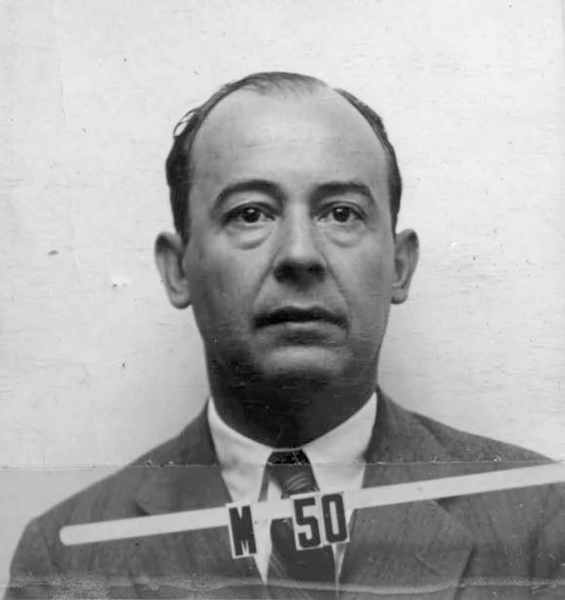
\includegraphics[scale=3]{imagenes/neumann.png}
\caption{John Von Neumann}
\label{fig:neumann}
\end{wrapfigure}
autoreplicarse, es decir, robots que se pudiera reproducirse a si mismos, pero pronto se dio cuenta de la altísima dificultad que suponía crear un robot que pudiera crear a su vez otros robots. La máquina tendría un coste de prestaciones muy elevado y requeriría una infinidad de piezas para poder construirse. Ulam que estaba estudiando el crecimiento de los cristales utilizando una red de celosía como modelo, ayudo a Neumann con el problema que se le había presentado sugiriéndole que utilizara un sistema discreto para crear un modelo reduccionista de autoreplicación. Además Neumann leyó un documento de Simposio Hixon titulado ``The general and logical theory of automata'' el cual le sirvió para desarrollar y publicar su teoría de Autómatas Celulares en su trabajo \cite{Teoria_Von_neumann} a finales de los años 40. \\

Esta primera teoría les sirvió a Ulam y Neumann para crear un método que calcula el movimiento de liquido. El concepto fundamental del método fue tratar el liquido como un conjunto de unidades discretas, finito y muy grande de pequeños elementos más simples cuyo comportamiento dependía de los elementos que lo rodeaban de esta forma se creó el primer autómata celular en la década de los cincuenta. Al igual que la red de celosía que estudiaba Ulam, los Autómatas Celulares de Neumann son bidimensionales, con su autoreplicación implementado de forma algorítmica. El resultado fue un autómata celular que en su interior creaba copias dentro de su sistema y con 29 estados por célula, de esta forma dio una prueba de la existencia de un patrón que podría hacer infinidad de copias de sí mismo dentro del su propio universo de células. Este diseño se le llamo ``constructor universal de Von Neumann''.\\

A partir de entonces los Autómatas Celulares fueron amplia mente estudiados por por varios científicos de la época.
En la década de 1960, fueron estudiados como un tipo particular de sistema dinámico y se estableció también una conexión con el campo matemático de la dinámica simbólica. En 1969, Gustav A. Hedlund realizo una compilación de estudios matemáticos de los Autómatas Celulares, un documento fundamental a partir de entonces. El resultado más importante fue la caracterización en el teorema de Curtis-Hedlund-Lyndon del conjunto de reglas globales de los Autómatas Celulares como el conjunto de continuos endomorfismos de espacios de turno.\\

También en 1969 el informático Alvy Ray Smith\cite{alvy} completó una tesis doctoral de Stanford en Teoría de Autómatas Celulares, el primer tratamiento matemático de los Autómatas Celulares enfocado al mundo de la ciencia de la computación y a los ordenadores en general. Muchos artículos posteriores vinieron de esta tesis: Mostró la equivalencia de los vecindarios de diversas formas, como reducir una vecindad de Moore a una vecindad de Von Neumann o cómo reducir cualquier zona de una vecindad de Von Neumann.


%--------------------------------------------------------------------------
%	Era de John Horton Conway
%--------------------------------------------------------------------------

\subsection{Era de John Horton Conway} % 
Los autómatas celulares tuvieron una gran expansión gracias a \textit{John Horton Conway} que en 1970 dio a conocer el autómata celular que probablemente sea el más conocido: el Juego de la vida (Life), publicado por Martin Gardner en su columna ``Mathematical Games'' en la revista ``Scientific American''. El Juego de la Vida consiste en una cuadrícula bidimensional con dos estados donde se coloca al inicio un patrón de células ``vivas'', representadas por una celda de color negro o ``muertas'', representadas por una celda de color blanco. 

\begin{figure}[H]
\centering
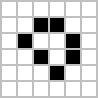
\includegraphics[scale=0.6]{imagenes/life_1.png}
\hspace{2cm}
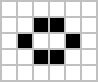
\includegraphics[scale=0.6]{imagenes/life_2.png}
\caption{Ejemplos de patrones del Juego de la Vida}
\label{fig:patrones}
\end{figure}


La vecindad para cada célula son ocho: los vecinos formados por la vecindad de  Moore. De manera repetida, se aplican simultáneamente sobre todas las células de la cuadrícula las siguientes 3 reglas:

\textit{Nacimiento}: se reemplaza una célula muerta por una viva si dicha célula tiene exactamente 3 vecinos vivos.\\
\textit{Muerte}: se reemplaza una célula viva por una muerta si dicha célula no tiene más de 1 vecino vivo (muerte por aislamiento) o si tiene más de 3 vecinos vivos (muerte por sobrepoblación).\\
\textit{Supervivencia}: una célula viva permanecerá en ese estado si tiene 2 o 3 vecinos vivos.\\

El juego hizo inmediatamente famoso Conway, pero también abrió un nuevo campo de investigación matemática en el campo de los autómatas celulares. Debido a las analogías de la vida con el ascenso, caída y transformaciones de una sociedad de organismos vivos, que pertenece a una creciente clase de juegos denominados "juegos de simulación" (juegos que se asemejan a los procesos de la vida real).\\

A pesar de su simplicidad, el sistema logra una impresionante diversidad de comportamientos, fluctuando entre aparente aleatoriedad y el orden. Una de las características más evidentes de juego de la vida es la frecuente aparición de planeadores o ``Gliders'', que son un tipo de patrón que se desplaza por la cuadrícula de forma continua , los arreglos de células que se mueven esencialmente a sí mismos a través de la rejilla. Es posible disponer el autómata para que los planeadores interactúen para realizar cálculos, y después de mucho esfuerzo se ha demostrado que el juego de la vida puede emular  la máquina de Turing.

\begin{figure}[H]
\centering
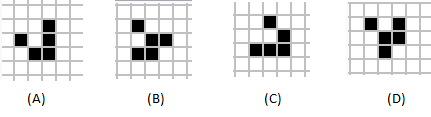
\includegraphics[scale=1]{imagenes/planeador.png}
\caption{Patrón planeador en sus cuatro generaciones}
\label{fig:planeador}
\end{figure}



%--------------------------------------------------------------------------
%	Era de Stephen Wolfram
%--------------------------------------------------------------------------

\subsection{Era de Stephen Wolfram} % 
\textit{Stephen Wolfram} comenzó a trabajar de forma independiente en autómatas celulares a mediados de 1981, después de considerar cómo los patrones complejos aparecían en la naturaleza. 
\begin{wrapfigure}{l}{0.4\linewidth}
\centering
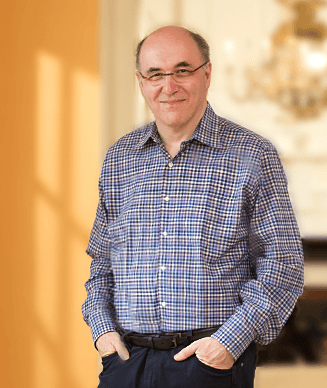
\includegraphics[scale=0.3]{imagenes/stephen.png}
\caption{Stephen Wolfram}
\label{fig:Stephen}
\end{wrapfigure}
Sus investigaciones fueron impulsadas inicialmente por un interés en los sistemas de modelado, tales como las redes neuronales. Él publicó su primer artículo en ``Reviews of Modern Physics'' donde investiga los autómatas celulares elementales ( Regla 30 en particular) en junio de 1983. La inesperada complejidad del comportamiento de estas reglas simples llevó a \textit{Wolfram} a sospechar que la complejidad en la naturaleza puede ser debido a mecanismos similares. Durante este período de \textit{Wolfram} formuló los conceptos de la intrínseca aleatoriedad y la irreductibilidad computacional , y sugirió que la regla 110 puede ser universal, hecho fue demostrado por asistente de investigación Mateo Cook, en la década de 1990. Durante su investigación tras múltiples simulaciones de diferentes Autómatas Celulares, estableció la siguiente clasificación de los mismos en virtud del comportamiento manifestado en los diagramas de evolución \cite{wolfram}:
\begin{itemize}
\item \textit{Autómata Celular de Clase 1}: son aquellos que evolucionan a estados homogéneos o constantes, es decir, o todo ceros, o todo unos. Además, dicha evolución es independiente de la configuración inicial considerada.
\item \textit{Autómata Celular de Clase 2}: son los autómatas que dan lugar a conjuntos de estructuras periódicas y estables. En ellos la evolución del estado de una determinada célula a lo largo del tiempo estará influida por los estados de un grupo fijo de células de la configuración inicial.
\item \textit{Autómata Celular de Clase 3}: son todos aquellos autómatas celulares cuyo comportamiento se vuelve caótico con el paso del tiempo, de tal forma que el cambio de estado de una célula va a depender cada vez más de una mayor número de estados iniciales. Se ha conjeturado que el cálculo de dichos estados se puede hacer mediante un simple algoritmo
\item \textit{Autómata Celular de Clase 4}: son aquellos que dan lugar a estructuras complejas, las cuales pueden permanecer localizadas en el espacio o bien moverse a lo largo del mismo. Es esta clase, la evolución del estado de una célula en particular dependerá de una gran cantidad de estados iniciales, de manera que la determinación exacta de dicho estado es un problema cuya complejidad es equivalente a la propia simulación explicita del Autómata Celular.
\end{itemize}

\begin{figure}[H]
\centering
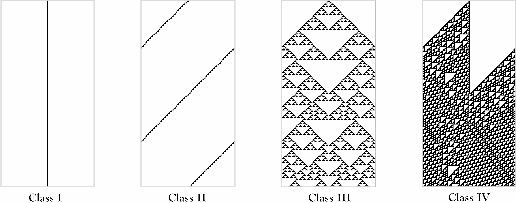
\includegraphics[scale=0.7]{imagenes/AutomatasCelulares_WolframClasses.png}
\caption{Ejemplos de Autómatas Celulares de cada clase.}
\label{fig:clase}
\end{figure}

En la figura superior se puede apreciar claramente de forma visual los tipos de clases que estableció \textit{Wolfram}


%--------------------------------------------------------------------------
%	Reglas de AC 
%--------------------------------------------------------------------------

\section{Reglas del Autómata} % 
Wolfram también definió un sistema de reglas o de notación consistente en asignar un numero natural de 0 a 255 a un Autómata Celular de la siguiente forma.\\

Considerando el caso particular de los Autómatas Celulares definidos de modo que su conjunto de estados es $S = \mathbb{Z}_2$ y el radio de la vecindad es $r = 1$. Para este caso particular de un Autómata Celular, el número de reglas de transición existentes es, según se menciono en la definición, de $2^{2^{2r+1}} = 2^8 = 256$ reglas de transición. Dado que $r = 1$ la vecindad de una célula está formada por ella misma, la célula a su izquierda y la célula situada a su derecha. Como el conjunto de estados es $\mathbb{Z}_2$, los dos estados en que puede encontrarse una célula son 0 ó 1. Consecuentemente existen $2^3 = 8$ posibles configuraciones de la vecindad de una célula dada, a saber: \\
$$111 \qquad 110 \qquad 101 \qquad 100 \qquad 011 \qquad 010 \qquad 001 \qquad 000$$

El primer dígito de cada configuración representa el estado de la célula de la izquierda, el dígito centra el estado de la célula de cuya vecindad hablamos y el último dígito hace referencia al estado de la célula de la derecha. Es claro que toda regla de transición consiste en asignar a cada una de estas posibles configuraciones de la vecindad un elemento de $\mathbb{Z}_2$. El número a asignar a una regla de transición se calculará de la siguiente forma:
\begin{enumerate}
 \item Se aplica la regla de transición a cada una de las 8 configuraciones anteriores,
 \item Se concatenan los bits obtenidos,
 \item Se interpreta dicha concatenación como un número en base 2 y
 \item Se considera la expresión decimal de dicho número.
\end{enumerate}

El número así obtenido se denomina el \textit{número de Wolfram} de la regla de transición considerada. Un ejemplo de esta regla sería:\\

Consideremos un Autómata Celular de $n = 11$ células, en el que $k = 2$ y $r = 1$. El conjunto de estado se este autómata celular es $\mathbb{Z}$ y la vecindad ya mencionada, además la regla de transición se rige por la siguiente expresión:
$$a_1^{t+1} = \lbrace a_{i-1}^t + a_{1}^t +a_{i+1}^t \rbrace mod 2, \qquad i \geq 0.  $$
Si el estado inicial del Autómata Celular es definido por la siguiente configuración
$$C^0 = (0,0,0,0,0,1,0,0,0,0,0)$$

calculando 8 generaciones sucesivas según la función de transición considerada, se obtiene la tabla de evolución siguiente:

\begin{figure}[H]
\centering
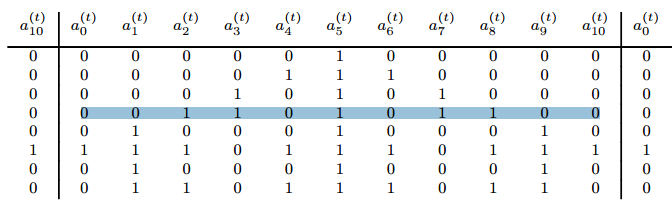
\includegraphics[scale=0.7]{imagenes/ejemplo_1.png}
\end{figure}

Ahora si se sustituye cada elemento numérico por un cuadrado de color dependiendo de si la célula esta viva, color negro, o muerta, color blanco, tal como se hacia en el juego de la vida de \textit{Conway}, se obtiene una tabla en la que se muestra el diagrama de evolución de este Autómata Celular para 8 generaciones

\begin{figure}[H]
\centering
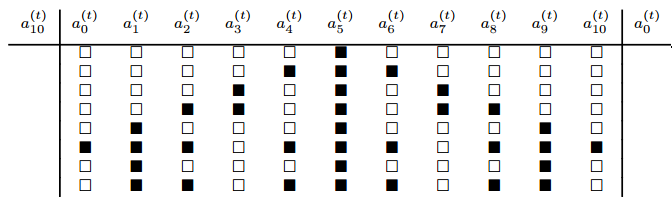
\includegraphics[scale=0.7]{imagenes/ejemplo_2.png}
\end{figure}

Para observar de forma más detallada la evolución de este Autómata Celular con la configuración inicial dada, se puede proceder a determinar, por ejemplo, las 50 primeras iteraciones. Llevando a cabo un proceso similar al anterior, de modo que sustituimos los 0 y 1 por cuadrados blancos y negros, obteniendo un diagrama de evolución como el de la siguiente figura:
 
\begin{figure}[H]
\centering
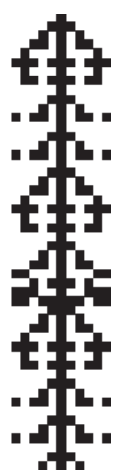
\includegraphics[scale=0.7]{imagenes/ejemplo_3.png}
\end{figure}



%--------------------------------------------------------------------------
%	Aplicaciones Actuales 
%--------------------------------------------------------------------------

\section{Aplicaciones Actuales} % 
Las aplicaciones de la teoría de autómatas celulares abarcan aspectos de la ciencia muy diversos como la computación e inteligencia artificial, la criptografía, el comportamiento de las moléculas de un gas, el flujo de tráfico y peatones, la evolución de la población, etc.

\subsection{Criptografía}
En al actualizada, la gran cantidad de información transmitida mediante redes de ordenadores y, en la mayoría de los casos, la necesidad de su confidencialidad, como por ejemplo: datos personales, cuentas bancarias, etc, hace necesario que esta información se transmita de manera fiable y segura. Está seguridad requiere del diseño e implementación de protocolos que garanticen la seguridad de los datos, de aquí nace la criptografía. El proceso de cifrar un mensaje consiste en transformarlo mediante un algoritmo de modo que sólo quien esté autorizado podrá invertir el proceso de cifrado para así poder obtener el mensaje original. Existen diversas formas de cifrar un mensaje y múltiples protocolos encargados de ello. Algunas de las técnicas de cifrado requieren una secuencia de bits pseudoaleatorios, para poder generar una clave de encriptado aparentemente aleatoria y sin ningún sentido pero que realmente si tiene una procedencia pre establecida y conocida. Para ello los Autómatas Celulares de Wolfram son excelentes como cifradores en flujo.\\

Consideremos los Autómatas Celulares de Wolfram definidos por las reglas de transición números 30 y 45, respectivamente, que parecen ser los que tienen mejores propiedades como generadores de bits pseudoaleatorios:
$$a_i^{t+1}  =  \lbrace a_{i-1}^t + a_i^t + a_{i+1}^t + a_i^t * a_{i+1}^t \rbrace \enspace  mod\enspace 2\enspace = a_{i-1}^t  \enspace XOR \enspace \big( a_i^t \enspace OR \enspace a_{i+1}^t \big) $$ 
$$a_i^{t+1}  =  \lbrace 1 + a_{i-1}^t + a_{i+1}^t + a_i^t * a_{i+1}^t \rbrace \enspace  mod\enspace 2\enspace = a_{i-1}^t  \enspace XOR \enspace \big( a_i^t \enspace OR \enspace \big( \enspace NOT \enspace a_{i+1}^t \big)\big) $$ 

Los diagramas de evolución de cada uno de los dos Autómatas Celulares anteriores pueden verse en las siguientes figuras:

\begin{figure}[H]
\centering
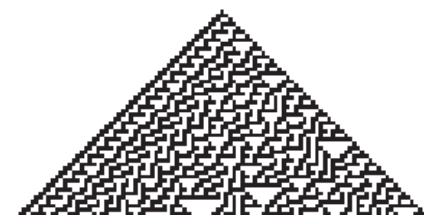
\includegraphics[scale=0.7]{imagenes/regla_30.png}
\caption{Diagrama de evolución del Autómata Celular de regla 30}
\end{figure}


\begin{figure}[H]
\centering
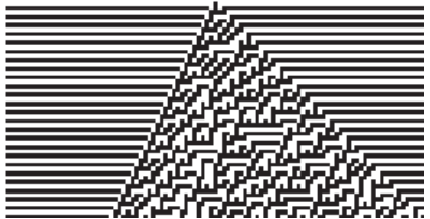
\includegraphics[scale=0.7]{imagenes/regla_45.png}
\caption{Diagrama de evolución del Autómata Celular de regla 45}
\end{figure}

Para este diagrama se han considerado 50 generaciones para cada autómata celular con la misma configuración inicial. Se podría pensar en utilizar estos dos Autómatas Celulares como generadores pseoudoaleatorios sin más que considerar como semilla a la configuración inicial y tomar como salida la lista de ceros y unos definida por la última configuración. Sin embargo, hacerlo así supondría que se generaría una lista de tantos bits  como bits de partida, dado que el número de células de todas las configuraciones es el mismo, por lo que este procedimiento no parece adecuado. Si lo que se desea es obtener una secuencia de bits cuya longitud sea mucho mayor que la longitud de la semilla o configuración inicial, es conveniente considerar como secuencia de salida la evolución de una de las células del Autómata. Con ello sólo haría falta conocer el estado inicial de unas pocas células e iterar el Autómata Celular tantas veces como bits se requieran.\\

Si se considera como salida del Autómata Celular la evolución de la célula central, sin considerar su estado inicial, a lo largo de 100 iteraciones, para la configuración inicial dada por:
$$(0,0,0,0,0,0,0,0,0,0,0,0,1,0,0,0,0,0,0,0,0,0,0,0,0,0)$$
se tiene la siguiente salida de 100 bits:
$$(1,0,1,1,1,0,0,1,1,0,0,0,1,0,1,1,0,0,1,0,0,1,1,1,1,0,$$
$$1,1,1,1,0,1,0,1,1,1,1,0,1,0,1,0,0,1,0,0,0,1,0,1,1,1,0,$$
$$0,0,0,0,1,0,0,1,1,0,1,1,1,1,1,0,0,1,0,0,1,0,0,1,0,0,$$
$$1,0,1,1,1,1,0,1,0,1,1,1,0,0,1,0,1,0,1,0,0)$$

Y su diagrama de evolución de la célula central, girado 90 grados, tiene la siguiente forma:

\begin{figure}[H]
\centering
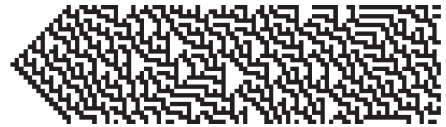
\includegraphics[scale=0.7]{imagenes/regla_30_100.png}
\caption{Diagrama de evolución del Autómata Celular de regla 30 con 100 iteraciones}
\end{figure}

Se puede observar que con la configuración inicial de 25 células dada anteriormente, se ha obtenido la secuencia de 100 bits presentada en antes, si bien esta longitud podría ser mucho mayor sin más que iterara más veces la evolución del Autómata Celular. La decisión de la secuencia de bits a utilizar como salida dependerá del tipo de Autómata Celular de que se trate. Téngase en cuanta que existen Autómatas Celulares cuya evolución es muy simétrica, lo que dificulta su uso como generadores de números pseudoaleatorios.\\

El proceso para escriptar un mensaje utilizando la generación de pseudoaleatorios sería el siguiente. Primero definimos un Autómata Celular, indicamos el patrón inicial que tendrá y generamos una salida de bits deseada, como hicimos anteriormente con las 100 iteraciones del Autómata Celular. Ahora concatenamos el valor en binario de cada una de las letras del mensaje, según su código ASCII, y luego sumar, bit a bit, el mensaje obtenido con la secuencia de bits generada. Por ejemplo la palabra "SECRETO" utilizando el Autómata anterior sería:

\begin{figure}[H]
\centering
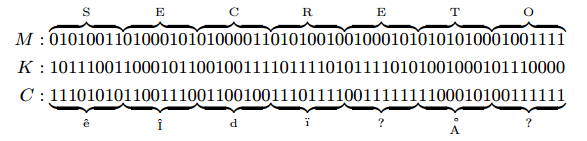
\includegraphics[scale=0.7]{imagenes/secreto.png}
\end{figure}

El destinatario para poder recuperar el mensaje original solo necesita concatenar el valor en binario de cada una de las letras o símbolos del criptograma recibido y sumar, bit a bit, el criptograma con la clave, realizando así una involución del mensaje.\\

La seguridad de este criptosistema está basada en la impredecibilidad de la clave, es decir, en la dificultad de poder obtener la secuencia pseudoaleatoria generada por el Autómata Celular. De ahí la importancia de que los Autómatas Celulares elegidos como generadores de bits pseudoaleatorios tengan buenas propiedades estadísticas. Hay estudios donde se comprueba y se revisa la seguridad de estos criptosistemas.\\



\subsection{Modelado de flujo de tráfico y peatones}

\subsection{Modelado de evolución de células o virus}

%------------------------------------------------

\bibliography{citas} %archivo citas.bib que contiene las entradas 
\bibliographystyle{plain} % hay varias formas de citar

\end{document}



